\documentclass[10pt,a4paper]{article}
\usepackage[margin=17mm]{geometry}
\usepackage[T1]{fontenc}
\usepackage[utf8]{inputenc}
\usepackage{lmodern,amsmath,amssymb,booktabs,graphicx,array,caption,float}
\usepackage[colorlinks=true,linkcolor=blue,citecolor=blue,urlcolor=blue]{hyperref}
\usepackage{microtype}
\graphicspath{{../figures/}}
\captionsetup{font=small,labelfont=bf}
\setlength{\parindent}{0pt}
\setlength{\parskip}{3pt}
\setlength{\abovecaptionskip}{5pt}
\newcommand{\Pa}{P_a}
\newcommand{\Rz}{R_0}
\newcommand{\Mw}{M_w}
\newcommand{\eqError}{0}
\newcommand{\eqSpeed}{1.09\times 10^{-14}}
\newcommand{\eqResidual}{-7.28\times 10^{-12}}
\newcommand{\pgInitial}{123232.667}
\newcommand{\naturalFreq}{589.70}
\newcommand{\strongCollapseTime}{54.763518}
\newcommand{\strongCollapseDuration}{5.278}
\newcommand{\strongExpansionDuration}{15.315}
\newcommand{\strongMach}{329.42}
\newcommand{\linearLow}{1.99\times 10^{-7}}
\newcommand{\linearHigh}{4.97\times 10^{-6}}
\newcommand{\convergedDiff}{5.66\times 10^{-10}}
\newcommand{\radauDiff}{4.35\times 10^{-10}}
\newcommand{\convergedOnebarDiff}{1.52\times 10^{-11}}
\newcommand{\radauOnebarDiff}{8.32\times 10^{-11}}
\newcommand{\minStrongStep}{1.80\times 10^{-15}}

\title{\vspace{-14mm}\Large\bfseries Mini-Research 1: Mathematical Modeling of\par Single-Bubble Dynamics under Acoustic Excitation}
\author{Dimitri Bolt}
\date{30 October 2026\\\small Preliminary manuscript for academic review; stage not closed}
\begin{document}
\maketitle
\vspace{-7mm}
\begin{abstract}
I compute five-cycle radius and wall-velocity trajectories for a spherical gas bubble in water driven at 30 kHz, using the incompressible Rayleigh--Plesset equation and constant polytropic exponent. Six amplitudes from 0 to 1.3 bar are checked by equilibrium, forcing phase, tolerance refinement, an independent integrator and the analytic linear limit. The 1.3 bar calculation produces physically inadmissible speeds, separating numerical convergence from physical validity. No bubble temperature is calculated.
\end{abstract}

\section{Introduction and scope}
Acoustic rarefaction expands a gas bubble; subsequent compression drives inward motion and rebound. Sadighi-Bonabi and Gheshlaghi~\cite{sadighi} supply the reference water radius and frequency, but their compressible and thermodynamic models are not replicated. Flannigan and Suslick~\cite{flannigan} report spectroscopic evidence associated with cavitation in concentrated aqueous sulfuric acid. That experiment motivates this work without quantitatively validating the water model.

The broader project includes later thermal and optical extensions. Here I restrict the study to deterministic radius dynamics: no laser, nanoparticle, gas energy, chemistry, nuclear-reaction or neutron calculation is included. Five cycles do not establish a stable periodic state.

\begin{figure}[H]
\centering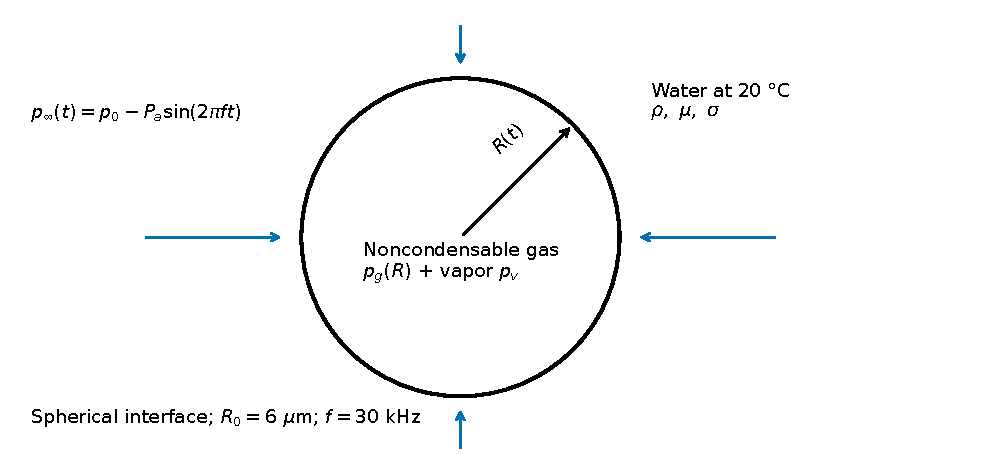
\includegraphics[width=.66\linewidth]{01_bubble_schematic.pdf}
\caption{Spherical bubble, interior pressure components, and acoustic forcing. The drawing is schematic and not to scale.}
\end{figure}

\section{Mathematical model}
The liquid is unbounded, spherical, incompressible and Newtonian, with constant density $\rho$, dynamic viscosity $\mu$, and surface tension $\sigma$. The radius is $R(t)>0$, in metres. The wall velocity is $\dot R$ in m/s. Spatially uniform gas pressure is represented by a constant-exponent closure, and the vapor partial pressure $p_v$ is held fixed:
\begin{equation}\label{eq:rp}
\rho\left(R\ddot R+\frac32\dot R^2\right)
=p_g(R)+p_v-p_\infty(t)-\frac{2\sigma}{R}-\frac{4\mu\dot R}{R},\qquad
p_g(R)=p_{g0}\left(\frac{R_0}{R}\right)^{3\kappa}.
\end{equation}
Here $p_g$ is the noncondensable-gas partial pressure; $p_g+p_v$ is the total internal pressure. The far-field absolute pressure is
\begin{equation}\label{eq:drive}
p_\infty(t)=p_0-\Pa\sin(2\pi f t),\qquad \Pa\geq0,\qquad T=1/f.
\end{equation}
All pressure variables are in Pa. The minus sign makes the first quarter-cycle a rarefaction. The initial state is $R(0)=R_0$, $\dot R(0)=0$.

\newpage
\subsection{Equilibrium and reduction to a first-order system}
At zero drive a static bubble has $R=R_0$, $\dot R=\ddot R=0$. Substitution into Eq.~\eqref{eq:rp} gives
\begin{align}
0&=p_g(R_0)+p_v-p_0-\frac{2\sigma}{R_0},\\
p_g(R_0)&=p_{g0},\qquad
\boxed{p_{g0}=p_0+\frac{2\sigma}{R_0}-p_v.}\label{eq:pg0}
\end{align}
The surface-pressure contribution is $2\sigma/R_0=24246.667$ Pa. Thus $p_{g0}=\pgInitial$ Pa is positive. The gas pressure excludes the vapor pressure so that vapor is not counted twice. Every term of Eq.~\eqref{eq:pg0} is a pressure, since $[\sigma/R]=({\rm N/m})/{\rm m}={\rm Pa}$.

To isolate the acceleration, subtract $3\rho\dot R^2/2$ from Eq.~\eqref{eq:rp}, divide by $\rho R$, and substitute the two pressure expressions:
\begin{align}
\rho R\ddot R&=p_g(R)+p_v-p_\infty(t)-\frac{2\sigma}{R}
-\frac{4\mu\dot R}{R}-\frac32\rho\dot R^2,\\
\ddot R&=\frac{p_g(R)+p_v-p_\infty(t)-2\sigma/R-4\mu\dot R/R}{\rho R}
-\frac{3\dot R^2}{2R}.
\end{align}
Define $U(t)=\dot R(t)$. Then $\dot U=\ddot R$, and the integrated system is exactly
\begin{equation}\label{eq:system}
\boxed{\begin{aligned}
\dot R&=U,\\
\dot U&=\frac{1}{\rho R}\left[
p_{g0}\left(\frac{R_0}{R}\right)^{3\kappa}+p_v-p_0+\Pa\sin(2\pi f t)
-\frac{2\sigma}{R}-\frac{4\mu U}{R}\right]-\frac{3U^2}{2R}.
\end{aligned}}
\end{equation}
The second-order initial conditions therefore become $(R,U)(0)=(R_0,0)$. Equilibrium also implies zero initial acceleration at $t=0$ for every amplitude, since $\sin0=0$; this does not imply zero motion at later times.

\subsection{Dimensional consistency}
The quantities $(R_0/R)^{3\kappa}$ and $\sin(2\pi f t)$ are dimensionless. Each bracketed term in Eq.~\eqref{eq:system} has pressure units. In particular,
\[
\left[\frac{\mu U}{R}\right]
=({\rm Pa\,s})\frac{{\rm m/s}}{{\rm m}}={\rm Pa},\qquad
[\rho R]=({\rm kg/m^3}){\rm m}={\rm kg/m^2}.
\]
Consequently $[{\rm Pa}/(\rho R)]={\rm m/s^2}$, while $[U^2/R]={\rm m/s^2}$. Both contributions to $\dot U$ are accelerations. On the original left-hand side $\rho R\ddot R$ and $\rho\dot R^2$ are both pressures. Here $\mu$ is explicitly \emph{dynamic} viscosity; kinematic viscosity would have units m$^2$/s and would require an extra density factor.

\subsection{Independent small-displacement limit}
Let $R=R_0(1+\varepsilon)$, with $|\varepsilon|\ll1$. To first order,
\[
p_g=p_{g0}(1-3\kappa\varepsilon),\quad
\frac{2\sigma}{R}=\frac{2\sigma}{R_0}(1-\varepsilon),\quad
\frac{4\mu\dot R}{R}=4\mu\dot\varepsilon,
\quad R\ddot R=R_0^2\ddot\varepsilon.
\]
Dropping products of perturbations, using Eq.~\eqref{eq:pg0}, and moving the restoring and damping terms left gives
\begin{equation}\label{eq:linear}
\rho R_0^2\ddot\varepsilon+4\mu\dot\varepsilon+
\left(3\kappa p_{g0}-\frac{2\sigma}{R_0}\right)\varepsilon
=\Pa\sin(2\pi f t),\quad \varepsilon(0)=\dot\varepsilon(0)=0.
\end{equation}
Its damped sinusoidal solution is evaluated analytically, independently of the nonlinear integrator. The undamped natural frequency is $f_0=\sqrt{(3\kappa p_{g0}-2\sigma/R_0)/(\rho R_0^2)}/(2\pi)=\naturalFreq$ kHz.

\newpage
\section{Physical parameters and numerical methods}
\begin{table}[H]
\centering\small
\caption{Fixed water-model parameters. Sources are direct references in the bibliography; all solver calculations use SI units. L: literature parameter; R: reference physical property; A: modeling assumption; D: derived parameter.}
\begin{tabular}{llll}
\toprule
Parameter & Model value & Class & Source or justification\\\midrule
$R_0$ & $6\times10^{-6}$ m & L & Ref.~\cite{sadighi}, Table II (water)\\
$f$ & $3.0\times10^4$ Hz & L & Ref.~\cite{sadighi}, Table II (water)\\
$T_{\ell}$ & 293.15 K (20 $^\circ$C) & L & Ambient water state, Ref.~\cite{sadighi}, Table II\\
$P_a$ & 0, 0.2, 0.5, 0.8, 1.0 bar & A & Prescribed amplitude study ($1$ bar $=10^5$ Pa)\\
$P_a$ & 1.3 bar & L & Additional case, Ref.~\cite{sadighi}, Table II\\
$p_0$ & 101325 Pa & A & Adopt standard atmosphere, Ref.~\cite{atm}\\
$\rho$ & 998.2 kg/m$^3$ & R & IAPWS-95, Ref.~\cite{iapws95}\\
$\mu$ & 0.001002 Pa\,s & R & IAPWS viscosity, Ref.~\cite{viscosity}\\
$\sigma$ & 0.07274 N/m & R & IAPWS surface tension, Ref.~\cite{surface}\\
$p_v$ & 2339 Pa & R & Saturation at 293.15 K, Ref.~\cite{iapws95}\\
$\kappa$ & 1.4 & A & Constant diatomic-gas adiabatic approximation\\
$c$ & 1482 m/s & R & IAPWS-95; diagnostic only, Ref.~\cite{iapws95}\\
$p_{g0}$ & $\pgInitial$ Pa & D & Static balance, Eq.~\eqref{eq:pg0}\\
$T$ & $3.333333\times10^{-5}$ s & D & $1/f$\\
$R_{\rm floor}$ & $6\times10^{-9}$ m & A & Technical termination, $0.001R_0$\\\bottomrule
\end{tabular}
\end{table}

I independently evaluated the IAPWS formulations using the open-source \texttt{iapws 1.5.4} implementation~\cite{implementation}. At 293.15 K and 0.101325 MPa, this gives $\rho=998.20715$ kg/m$^3$, $\mu=0.0010015961$ Pa\,s and $c=1482.3462$ m/s. Saturation values at that temperature are $p_v=2339.3182$ Pa and $\sigma=0.07273614$ N/m. The fixed rounded values above are retained for every amplitude; the small rounding of viscosity is about 0.040\%. Saturation surface tension is used as an approximation to the bubble interface value.

In contrast, Table I of Ref.~\cite{sadighi} lists water values $\sigma=0.038$ N/m, $\mu=1.307\times10^{-3}$ Pa\,s and $c=1660$ m/s. These differ materially from the independent reference evaluation and are not adopted. Its vapor pressure, 0.338 psi (about 2330 Pa), is close. The paper calls viscosity kinematic in Section II while its table uses Pa\,s; the units support interpreting that coefficient as dynamic viscosity. I do not infer a cause for these discrepancies.

\subsection{Adaptive integration and protection}
I integrate Eq.~\eqref{eq:system} over $0\leq t\leq5T=166.667$ \textmu s for $\Pa=0,0.2,0.5,0.8,1.0,1.3$ bar; 1 bar is $10^5$ Pa. The primary solver is SciPy's eighth-order DOP853~\cite{scipy}, appropriate for high-accuracy nonstiff trajectories, with $\mathrm{rtol}=10^{-10}$, separate absolute tolerances $(10^{-16}\ {\rm m},10^{-8}\ {\rm m/s})$, maximum step $T/1000$, and dense output. Radau supplies an independent implicit-method check of the same ODE.

A small DOP853 subclass rejects an internal trial with $R\leq0$ and retries at one quarter of the step; it never clips the state or modifies the force. This safeguard was needed in the coarse stress-test calculation. A decreasing-radius event terminates at $R_{\rm floor}$, and incomplete or unsuccessful production runs raise an error. A floor termination would censor the inferred minimum. None of the reported sweep runs reaches that floor.

Zeros of $U$ locate radius maxima/minima; zeros of $\dot U$ locate velocity extrema. The initial root is excluded from local-event counts. Roots on accepted-step dense output are refined by a bracketed solve with absolute time tolerance $10^{-24}$ s, rather than relying on SciPy's approximately $10^{-15}$ s default event tolerance. This matters for the formal sub-picosecond rebound; it is a numerical setting, not physical timing accuracy. Exported trajectories include adaptive-step subdivisions, all event times and a 5001-point common grid.

\newpage
\section{Results: finite-time radius response}
\begin{table}[H]
\centering\scriptsize
\caption{Extrema over five cycles, including endpoints. $U_+=\max(U,0)$ and $|U_-|=|\min(U,0)|$; $N_+,N_-$ count post-initial radius maxima/minima. Zero-drive speeds are roundoff. The 1.3 bar row is a formal ODE result outside physical validity.}
\resizebox{\linewidth}{!}{\begin{tabular}{rrrrrrr}
\toprule
$P_a$ (bar) & $R_{\max}$ (\textmu m) & $R_{\min}$ (\textmu m) & $U_+$ (m/s) & $|U_-|$ (m/s) & $M_{w,\max}$ & $N_+/N_-$ \\
\midrule
0.0 & 6.0000 & 6.00000 & 0 & 0 & 0 & 0/0 \\
0.2 & 6.2815 & 5.77656 & 0.08991 & 0.06694 & 6.07e-05 & 10/10 \\
0.5 & 6.8887 & 5.50864 & 0.2275 & 0.1856 & 0.000153 & 9/9 \\
0.8 & 8.0833 & 5.28189 & 0.3886 & 0.4185 & 0.000282 & 47/47 \\
1.0 & 11.3381 & 4.12142 & 7.477 & 7.737 & 0.00522 & 88/88 \\
1.3 & 65.7575 & 0.02533 & 4.881e+05 & 4.882e+05 & 329 & 27/27 \\
\bottomrule
\end{tabular}
}
\end{table}

At 0.2--0.8 bar the radius excursions are modest: rarefaction expands the bubble, compression reduces it, and the wall speed remains small. Increasing to 1.0 bar produces stronger asymmetry and rebound oscillations. Its radius lies between approximately 4.12 and 11.34 \textmu m; the largest wall speed is about 7.74 m/s. The corresponding wall Mach number is approximately 0.0052, so this particular compressibility diagnostic remains small. The first-order gas closure and other limitations still apply.

\begin{figure}[H]
\centering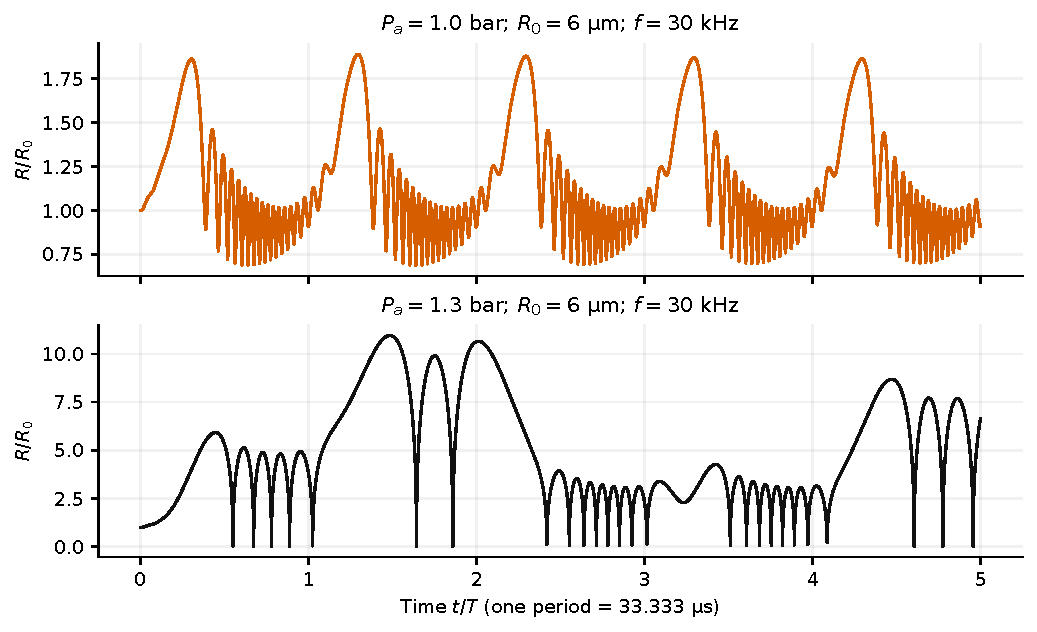
\includegraphics[width=.86\linewidth]{02_radius_vs_time.pdf}
\caption{Computed radius histories at 1.0 and 1.3 bar with identical physical parameters. The second panel illustrates the formal strong-collapse regime, whose extreme compressions cannot be interpreted as physical predictions. Small rebound oscillations are resolved by adaptive integration.}
\end{figure}

At 1.3 bar the polytropic incompressible model allows much greater expansion and a highly concentrated rebound. Both its extreme compression and its enormous wall speed are numerical properties of this model. With $\Mw\gg1$, the model has already lost the assumptions needed to interpret those values physically. I retain this row to expose the failure of applicability rather than silently remove the extreme result.

The phase trajectories (Appendix, Fig.~\ref{fig:phase}) contain expansion, inward acceleration and rebounds. The many local extrema in Table 2 reflect these rebounds as well as the driven response. Counts include small but resolved radius oscillations, with no amplitude threshold; they are not counts of acoustic cycles. The initial value $R(0)=R_0$ participates in global bounds but is not counted as a later local minimum.

The amplitude comparison and metric curves in the Appendix show increased excursion and rapid growth of wall speed toward the last amplitude. Connecting six computed amplitudes guides the eye; it does not identify a bifurcation threshold or establish a continuous transition curve. No long-time attractor, periodic orbit or shape stability is inferred from this five-cycle experiment.

\newpage
\section{Collapse timing and numerical verification}
For reproducibility I define the characteristic collapse time $t_c$ as the deepest post-initial local radius minimum within the simulation. Its collapse duration is $t_c-t_{\max}$, where $t_{\max}$ is the preceding local maximum. This differs from the empty-cavity Rayleigh collapse-time formula. The preceding expansion duration runs from the preceding local minimum (or $t=0$) to that maximum.

For the formal 1.3 bar stress test, $t_c=\strongCollapseTime$ \textmu s. The selected expansion and collapse intervals are $\strongExpansionDuration$ and $\strongCollapseDuration$ \textmu s, respectively. The most concentrated final rebound occupies a much shorter scale. The smallest accepted step is approximately $\minStrongStep$ s, so a few hundred equally spaced samples could not resolve it.
\begin{figure}[H]
\centering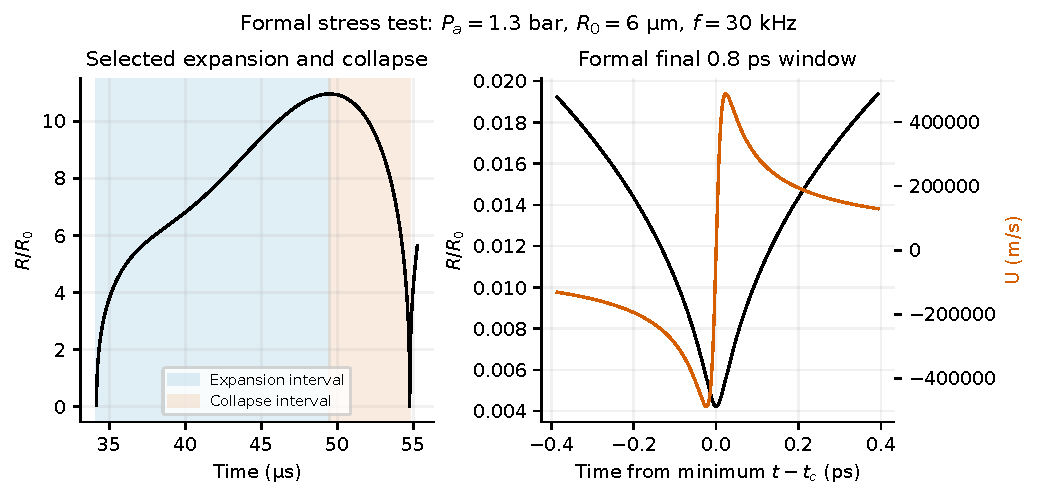
\includegraphics[width=.73\linewidth]{06_collapse_zoom.pdf}
\caption{Selected expansion--collapse interval and a final 0.8 ps view of the formal 1.3 bar solution. The speed uses the colored right axis. The severe time-scale separation is resolved numerically but occurs far outside incompressible physical validity.}
\end{figure}

\subsection{Equilibrium, phase and linear checks}
Analytically, $p_{g0}+p_v-p_0-2\sigma/R_0=0$. The floating-point residual is $\eqResidual$ Pa. The five-cycle numerical equilibrium error is
\[
E_{\rm eq}=\max_t\left|\frac{R-R_0}{R_0}\right|=\eqError<10^{-8},
\qquad \max|U|=\eqSpeed\ {\rm m/s}.
\]
At $\Pa=10^5$ Pa the pressure check gives $p_\infty(0)=101325$ Pa, $p_\infty(T/4)=1325$ Pa and $p_\infty(3T/4)=201325$ Pa, confirming the intended sign.

The nonlinear radius differs from the independent analytic solution of Eq.~\eqref{eq:linear} by $\linearLow R_0$ at 100 Pa and $\linearHigh R_0$ at 500 Pa. The approximately quadratic increase with amplitude is consistent with the neglected second-order terms. These small auxiliary amplitudes are independent tests, not replacements for the required sweep.

\subsection{Tolerance and second-method comparison}
\begin{table}[H]
\centering\scriptsize
\caption{Stress-test convergence at 1.3 bar. Maximum relative difference is over $R_{\max},R_{\min},t_c,|U|_{\max}$ against the fourth row. All runs finish five cycles. Full component tolerances and step caps are in \texttt{convergence.csv}.}
\resizebox{\linewidth}{!}{\begin{tabular}{lrrrrr}
\toprule
Method / rtol & $R_{\max}$ (\textmu m) & $R_{\min}$ (\textmu m) & $t_c$ (\textmu s) & $|U|_{\max}$ (m/s) & Max. rel. diff. \\
\midrule
DOP853 / $1.00\times 10^{-7}$ & 65.757536 & 0.0253271 & 54.7635171 & 488193.285 & $9.08\times 10^{-7}$ \\
DOP853 / $1.00\times 10^{-9}$ & 65.757544 & 0.0253271 & 54.7635179 & 488193.733 & $1.07\times 10^{-8}$ \\
DOP853 / $1.00\times 10^{-10}$ & 65.757544 & 0.0253271 & 54.7635179 & 488193.728 & $5.66\times 10^{-10}$ \\
DOP853 / $1.00\times 10^{-11}$ & 65.757544 & 0.0253271 & 54.7635179 & 488193.728 & $0$ \\
Radau / $1.00\times 10^{-10}$ & 65.757544 & 0.0253271 & 54.7635179 & 488193.728 & $4.35\times 10^{-10}$ \\
\bottomrule
\end{tabular}
}
\end{table}
The step caps are $T/100,T/300,T/1000,T/2000$ for the four DOP853 rows, with absolute tolerance pairs $(10^{-13},10^{-5})$, $(10^{-15},10^{-7})$, $(10^{-16},10^{-8})$, $(10^{-17},10^{-9})$ in m and m/s. Radau uses the third pair and $T/1000$. Production differs from the tighter reference by at most $\convergedDiff$ in these metrics; Radau differs by at most $\radauDiff$. This supplies a measured convergence check, not merely a successful solver status.

\newpage
\section{Physical applicability and relation to the publications}
The diagnostic $\Mw=|U|/c$ compares wall speed to liquid sound speed. Values of order 0.1 already warrant caution; values near unity invalidate the incompressible description of rapid wall motion. For 1.3 bar, the computed maximum is approximately $\strongMach$, an unequivocal failure of that assumption. The formal radius minimum remains above the technical 6 nm floor, but that fact supplies no physical credibility. At 1.0 bar and below, small wall Mach number removes this specific warning without validating the other assumptions.

The forcing itself has an additional limitation. Its minimum is $p_0-\Pa$. At 1.3 bar it is $-28675$ Pa, so the imposed far-field \emph{absolute} pressure is negative over part of each cycle. This corresponds to imposed tensile liquid stress in the model, not an admissible equilibrium gas pressure. Real cavitation nucleation and tensile stability are not determined here. No pressure clipping is used. At 1.0 bar the minimum remains positive, 1325 Pa.

The assumed water properties remain at their ambient values throughout motion. Constant $\kappa=1.4$ approximates adiabatic compression of a diatomic gas; it is neither a complete thermal model nor a measured effective exponent over the entire cycle. In particular, gas identity is not calibrated to the noble-gas contents of the experimental motivation. Thermal exchange during slow expansion could change the effective pressure law substantially. Fixed vapor pressure omits evaporation and condensation kinetics, while no mass transfer or gas diffusion changes the gas inventory. Spatially uniform gas pressure, spherical shape, an unbounded liquid, and the absence of shock waves, radiation damping and finite molecular excluded volume impose further restrictions. The present equations cannot evaluate shape-mode growth or shock formation, even when the radial ODE integrates smoothly.

\subsection{Why the classical equation is adequate for this stage}
Section II, Eqs.~(1)--(4) of Ref.~\cite{sadighi} includes finite-sound-speed terms multiplying acceleration and inertia, a pressure time derivative, and a van der Waals excluded-volume gas law. Its gas-pressure normalization also does not make the same explicit noncondensable-gas/vapor split as Eq.~\eqref{eq:pg0}. The quasi-adiabatic and hydro-chemical closures add physics absent here. Its Eq.~(4) writes the driving pressure with a positive sine, giving an external-pressure phase opposite to Eq.~\eqref{eq:drive}. Matching initial phase is therefore essential before comparing trajectories.

Table II of that paper gives the water case $R_0=6$ \textmu m, $f=30$ kHz and $\Pa=1.3$ bar. Table III uses the same water radius and frequency in a hydro-chemical calculation; Table IV instead gives a laser-assisted water case with $R_0=1.5$ \textmu m and $\Pa=1.4$ bar. Other rows concern deuterated acetone at different temperatures and frequencies. Their radius ratios cannot serve as quantitative targets for the present constant-exponent incompressible model with different reference properties. Flannigan and Suslick's sulfuric-acid spectra likewise provide motivation, not radius-trajectory validation in water.

The classical equation is sufficient to establish a transparent derivation, an equilibrium-consistent pressure law, adaptive integration, amplitude dependence and explicit validity diagnostics. A compressible description would be needed before interpreting the strongest collapse, but no second physical model is implemented here.

\section{Conclusions}
I obtained reproducible radius, wall-velocity and phase trajectories over five acoustic cycles, including expansion, collapse and rebounds. The equilibrium and forcing checks, independent linear limit, tolerance study and Radau comparison support numerical consistency. Greater drive increases radial excursions and can create extreme formal collapses whose apparent numerical convergence does not rescue physical validity.

The 1.0 bar solution has a maximum speed near 7.74 m/s, whereas the 1.3 bar stress test violates incompressibility by a very large margin and imposes negative far-field pressure during rarefaction. No reliable extreme-collapse temperature or fusion claim follows. The verified radius-model implementation provides a basis for later review of compressibility and gas-pressure closures; those extensions remain outside this study. This manuscript is prepared for independent review, and Mini-Research 1 remains open.

\newpage
\begin{thebibliography}{9}\small
\bibitem{sadighi} R. Sadighi-Bonabi and M. Gheshlaghi, ``Laser induced sonofusion: A new road toward thermonuclear reactions,'' \emph{AIP Advances} \textbf{6}, 035218 (2016). \href{https://doi.org/10.1063/1.4945343}{doi:10.1063/1.4945343}. Section II, Eqs.~(1)--(4); Tables I--IV.
\bibitem{flannigan} D. J. Flannigan and K. S. Suslick, ``Plasma formation and temperature measurement during single-bubble cavitation,'' \emph{Nature} \textbf{434}, 52--55 (2005). \href{https://doi.org/10.1038/nature03361}{doi:10.1038/nature03361}.
\bibitem{iapws95} IAPWS, \emph{R6-95(2018): Revised Release on the IAPWS Formulation 1995 for the Thermodynamic Properties of Ordinary Water Substance for General and Scientific Use} (2018). \url{https://iapws.org/technical-guidance/release/IAPWS-95}.
\bibitem{surface} IAPWS, \emph{R1-76(2014): Revised Release on the Surface Tension of Ordinary Water Substance} (2014), equation and Table 1. \url{https://iapws.org/technical-guidance/release/Surf-H2O}.
\bibitem{viscosity} IAPWS, \emph{R12-08: Release on the IAPWS Formulation 2008 for the Viscosity of Ordinary Water Substance} (2008). \url{https://iapws.org/technical-guidance/release/viscosity}.
\bibitem{implementation} J. J. G\'omez Romera and contributors, \emph{iapws}, Python implementation, version 1.5.4. \url{https://github.com/jjgomera/iapws}. Implementation documentation: \url{https://iapws.readthedocs.io/en/latest/iapws.iapws95.html}.
\bibitem{scipy} SciPy developers, \emph{solve\_ivp documentation}; numerical package version 1.16.3 used in this work. \url{https://docs.scipy.org/doc/scipy/reference/generated/scipy.integrate.solve_ivp.html}.
\bibitem{atm} BIPM, \emph{The International System of Units (SI)}, 9th ed., Appendix 1, 10th CGPM (1954), Resolution 4: standard atmosphere, 101325 Pa. \url{https://www.bipm.org/en/committees/cg/cgpm/10-1954/resolution-4}.
\end{thebibliography}

\section*{Reproducibility record}
The accompanying code uses Python 3.12.14, NumPy 2.3.5, SciPy 1.16.3, Matplotlib 3.10.7, pytest 8.4.2 and iapws 1.5.4. The README supplies environment creation, installation, simulation, plotting, test and LaTeX commands. Numeric report tables are generated from saved results; figures are regenerated without reintegrating. All physical and numerical inputs, source hashes and solver statistics are preserved in \texttt{results/run\_metadata.json}. Original source documents and the general project plan are unchanged.

The supplementary figures retain all six prescribed amplitudes and the validity warnings. The CSV files contain unrounded extrema; rounded printed values do not replace the numerical records. Tests include equilibrium, forcing phase, acceleration balance, invalid states and amplitudes, floor termination, the linear limit, and independent-method agreement.

\newpage
\appendix
\section{Wall velocity and phase trajectories}
\begin{figure}[H]
\centering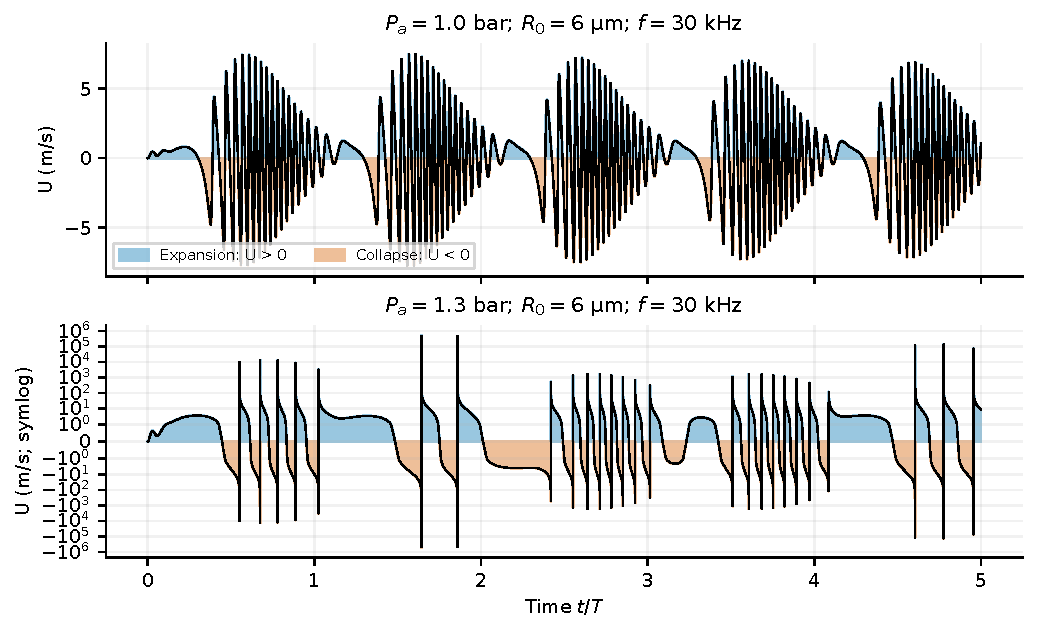
\includegraphics[width=.96\linewidth]{03_wall_velocity_vs_time.pdf}
\caption{Wall velocities at 1.0 and 1.3 bar. Positive and negative intervals indicate expansion and collapse. The symmetric logarithmic lower panel retains small motions and extreme formal speeds; the latter invalidate incompressible physical interpretation.}
\end{figure}
\begin{figure}[H]
\centering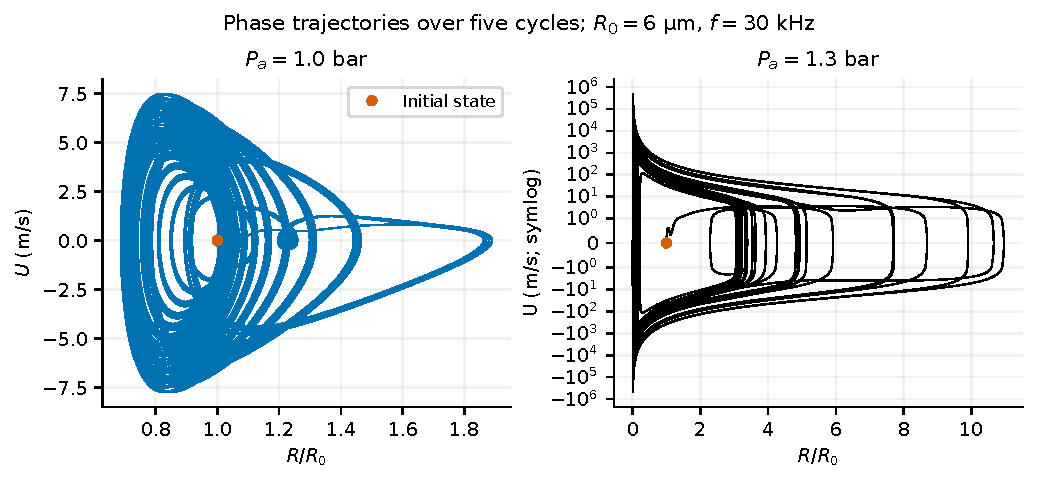
\includegraphics[width=.96\linewidth]{04_phase_portrait.pdf}
\caption{Five-cycle phase trajectories at 1.0 and 1.3 bar. Radius is normalized by $R_0$; speed remains dimensional. The marked point is the initial state, not a subsequent minimum. The second panel is outside physical validity.}\label{fig:phase}
\end{figure}

\newpage
\section{Amplitude dependence}
\begin{figure}[H]
\centering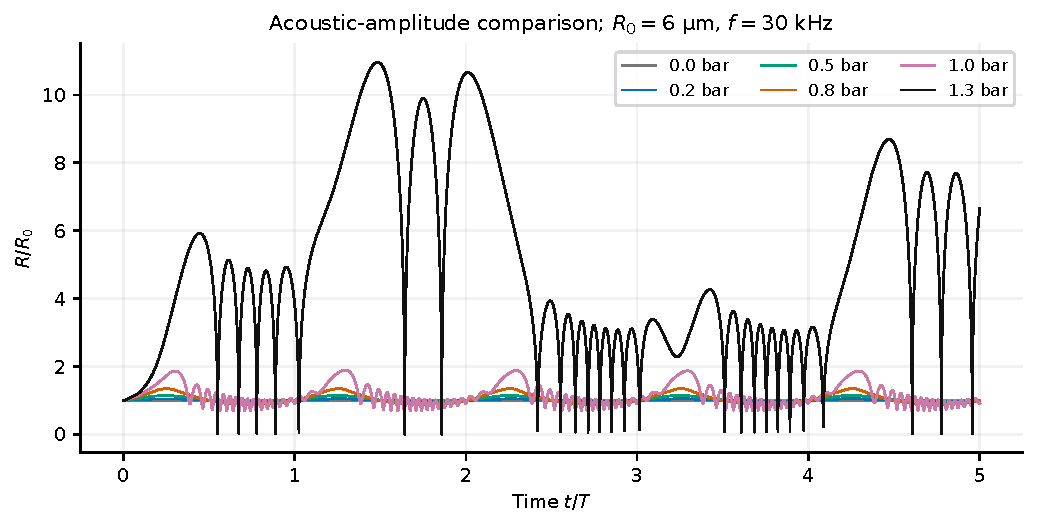
\includegraphics[width=.96\linewidth]{05_amplitude_comparison.pdf}
\caption{All six amplitude cases with fixed water properties, gas exponent, radius and frequency. The 1.3 bar case is retained as a formal stress test.}
\end{figure}
\begin{figure}[H]
\centering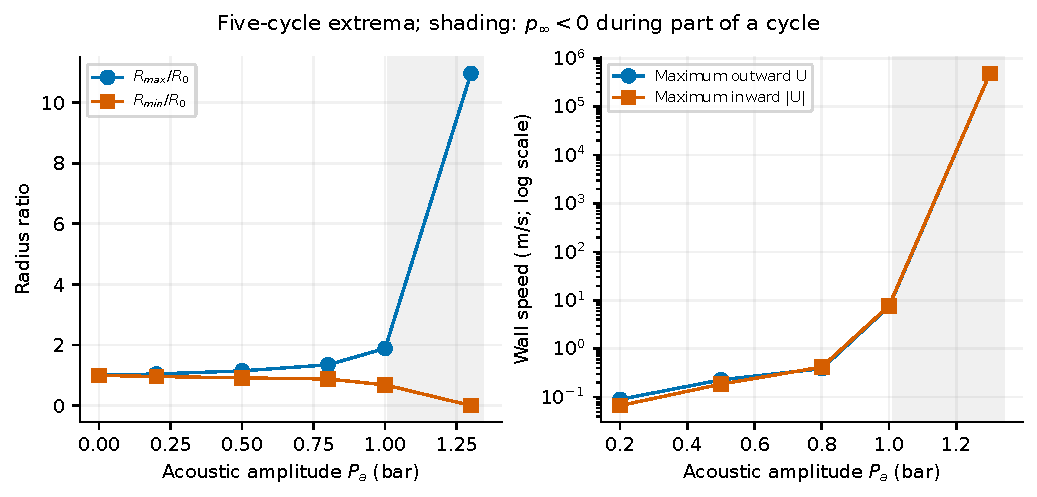
\includegraphics[width=.96\linewidth]{07_amplitude_sweep_metrics.pdf}
\caption{Global radius and speed extrema. The zero-drive speed is omitted from the logarithmic panel. Shading marks amplitudes at which the imposed far-field absolute pressure becomes negative during a cycle.}
\end{figure}

\newpage
\section{Convergence and validity diagnostics}
\begin{figure}[H]
\centering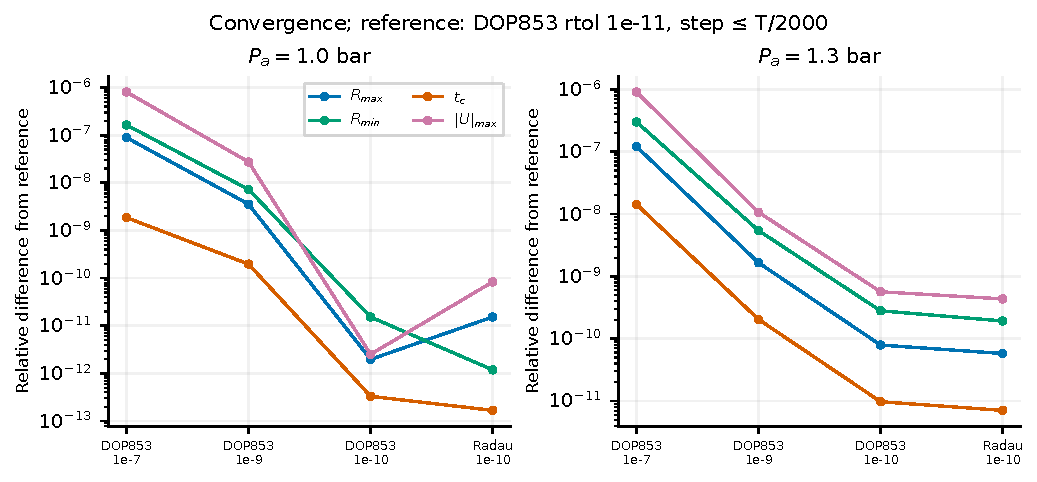
\includegraphics[width=.96\linewidth]{08_numerical_convergence.pdf}
\caption{Relative metric differences at 1.3 bar against the tighter DOP853 reference. Several tolerances and step caps, and a second method, measure numerical consistency of the formal ODE.}
\end{figure}
\begin{figure}[H]
\centering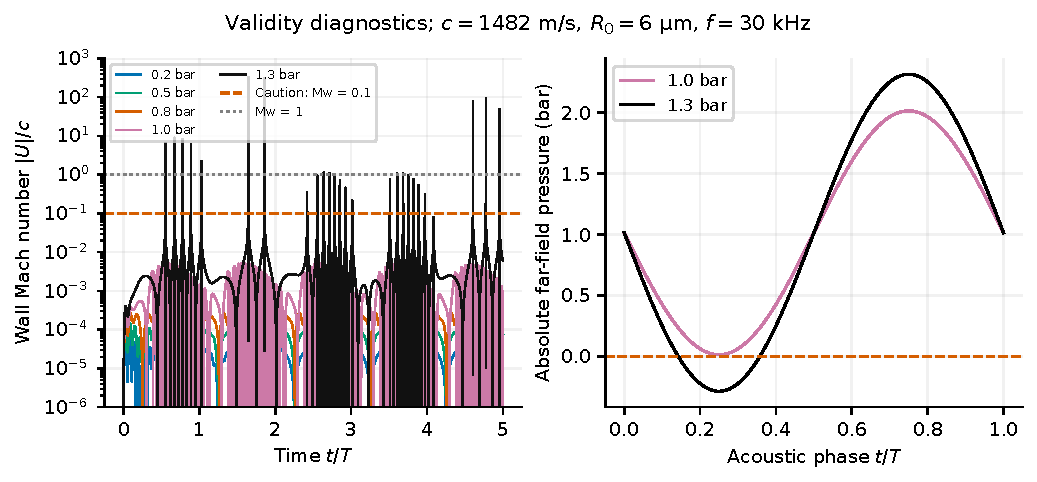
\includegraphics[width=.96\linewidth]{09_validity_diagnostics.pdf}
\caption{Wall Mach number and imposed pressure. The 1.3 bar trajectory exceeds both the caution level 0.1 and unity by large factors. Its far-field pressure is negative over part of rarefaction. The logarithmic Mach panel excludes zero values only for plotting.}
\end{figure}
\end{document}
